\documentclass[../dissertation.tex]{subfiles}
\begin{document}
Now that gradient flow equation and tangent-point energy are introduced,
one can formalise the process of untangling a tangled curve:

\begin{definition}[Curve Untangling Process]
    Given a parameterised curve $\gammabf:M \times T \rightarrow \mathbb{R}^3$ over an interval $M$ and time domain $T$,
    denote the following initial value problem as \textbf{curve untangling process}:
    \begin{align}
        \frac{\partial \gammabf}{\partial t} &= - \grad_{\mathcal{X}} \mathcal{E}_{\beta}^{\alpha} (\gammabf) - \grad_{\mathcal{X}} \mathcal{C} (\gammabf) 
        \label{equ: Curve Untangling Process}
        \\
        \gammabf(s;0) &= \gammabf_0 (s)
        \label{equ: Initial Curve}
    \end{align}
    where 
    \begin{itemize}
        \item $\gammabf_0 (s)$ is the parameterisation of the initial (tangled) curve (prescribed at $t=0$)
        \item $\mathcal{E}_{\beta}^{\alpha}$ is the tangent-point energy (See (\ref{equ: Tangent-Point Energy}))
        \item $\mathcal{C}$ is additional constraint energy to control behaviour of curve untangling process.
    \end{itemize}
\end{definition}

\subsection{Discretisation for Numerical Computation}
Solving (\ref{equ: Curve Untangling Process}), (\ref{equ: Initial Curve}) analytically is challenging.
Rather, we aim to acquire a numerical solution.
Assume for simplicity that the curve of interest is closed.
We start by discretising the initial curve $\gammabf_0$ by taking $N$ points on a curve as shown in Figure \ref{fig: Discretization of Curve}.
Represent the initially discretised curve as $\Gammabf^0 = \left( \xbf_0^0, \xbf_1^0, \cdots, \xbf_{N-1}^0 \right)$,
and the discretised curve at time step $k \in \mathbb{N} \cup \left\{ 0 \right\}$ as $\Gammabf^k = \left( \xbf_0^k, \xbf_1^k, \cdots, \xbf_{N-1}^k \right)$
and assign a function definition $\Gammabf^k: \mathbb{Z} \rightarrow \left\{ \xbf_0^k, \xbf_1^k, \cdots, \xbf_{N-1}^k \right\}$ as:
\begin{equation}
    \Gammabf^k (i) = \xbf_{r\left( i, N \right)}^k \hspace{1cm} \text{where } r\left( i,N \right) = \text{(remainder of } i \div N \text{)}
\end{equation}
\begin{figure}[tbp]
    \centering
    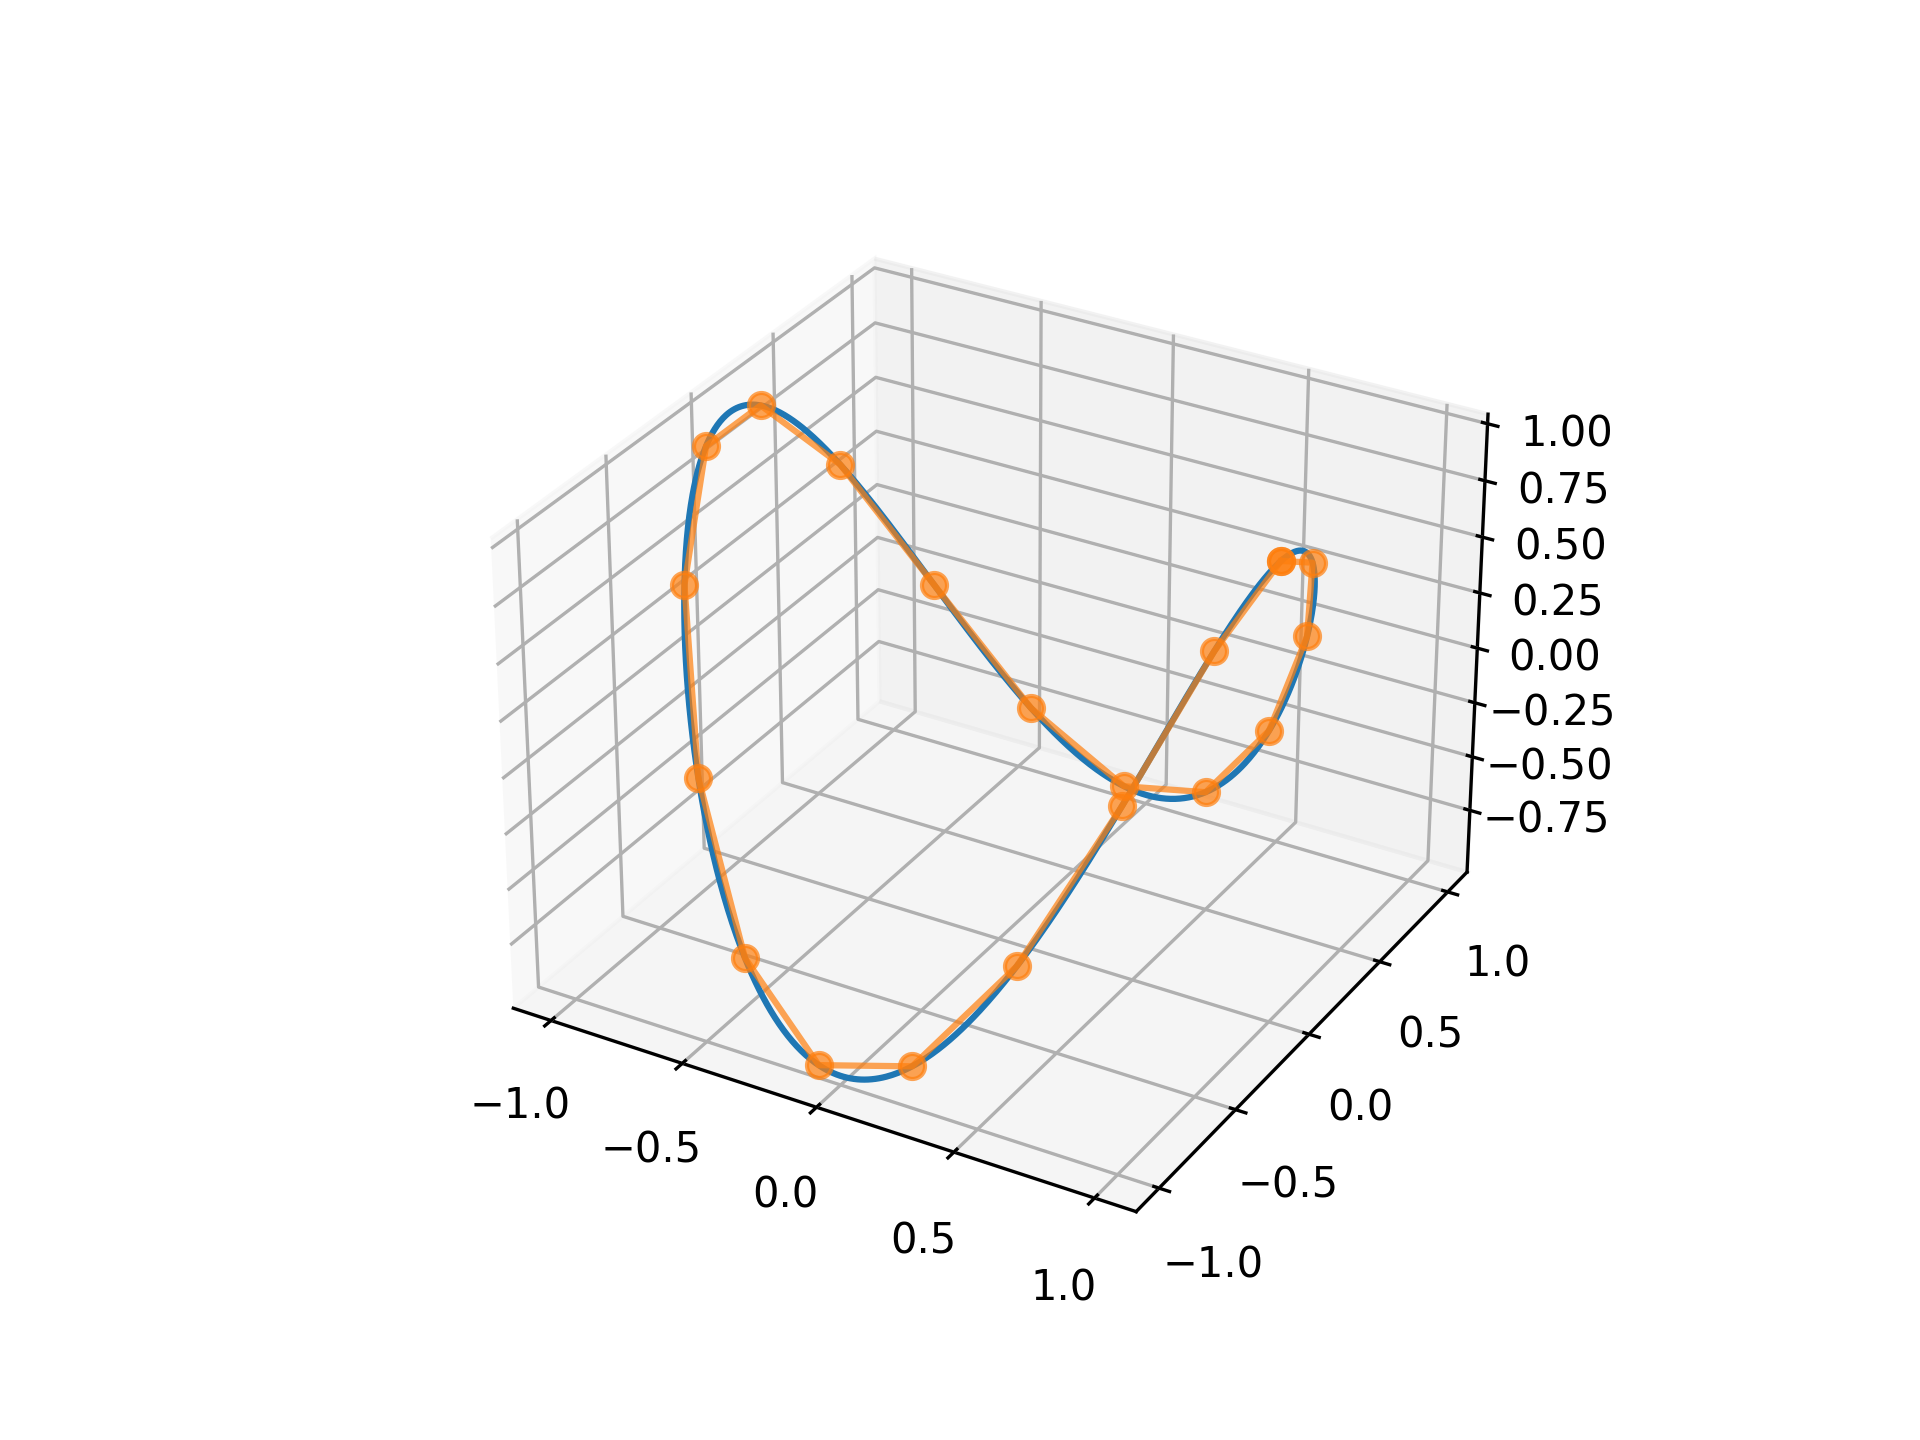
\includegraphics[width=0.8\textwidth]{sections/discretizationImgs/discretization}
    \caption{Discretisation of a closed curve by sampling the points along the curve.}
    \label{fig: Discretization of Curve}
\end{figure}

Based on (\ref{equ: Curve Untangling Process}), one writes the following finite difference scheme:
\begin{equation}
    \mathcal{D}_{t} \Gammabf^{k} = -\grad_{\mathcal{X}} E_{\beta}^{\alpha} (\Gammabf^k) - \grad_{\mathcal{X}} C \left( \Gammabf^k \right) \hspace{1cm} \text{for } k=0,1,\cdots
\end{equation}
where $\mathcal{D}_t$ is the finite difference operator over time step.

\end{document}
